\section{Façade}

Quando um subsistema possui muitas interfaces 
de acesso às suas funcionalidades, o acesso de 
classes clientes de outros subsistemas a ele 
torna-se descentralizado, aumentando a dependência 
entre os dois sistemas. Para minimizar esse problema, 
o padrão Façade fornece uma interface generalizada 
para todo o subsistema, de forma que as classes 
clientes possam comunicar-se apenas com um ponto 
de entrada. A figura \ref{facade_struct} demonstra 
o padrão, onde uma classe Façade, que é o ponto de 
acesso ao subsistema, possui uma referência para 
os componentes que antes eram diretamente acessíveis.

\begin{figure}[htb]
	\caption{\label{facade_struct}Estrutura do Façade}
	\begin{center}
	    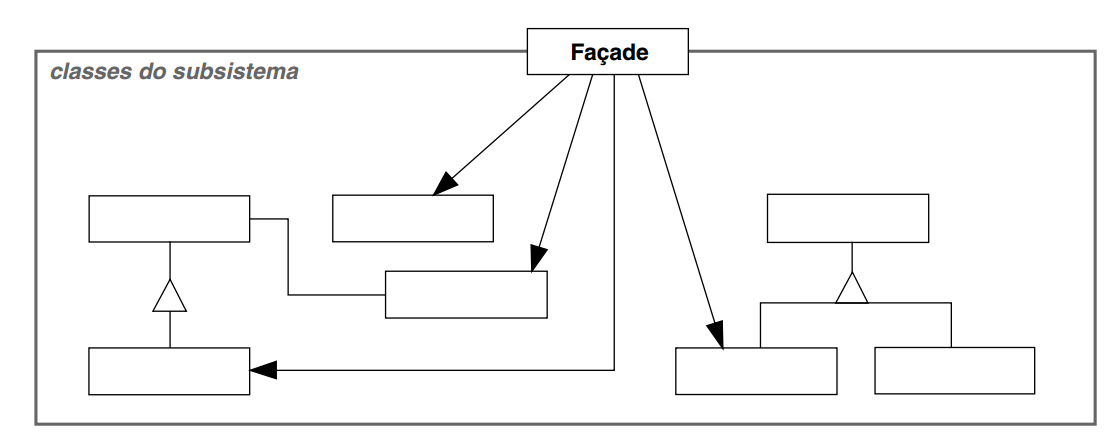
\includegraphics[scale=0.4]{5_padroes-contexto-funcional/5.2_estruturais/5.2.5_facade/diagram.png}
	\end{center}
\end{figure}

\subsection*{Exemplo Orientado a Objetos}

Como exemplo de uso do Façade, pode-se considerar 
um compilador que oferece diversas funcionalidades. 
Essas funcionalidades são apresentadas no diagrama 
de classes da figura \ref{facade_exemplo}, representadas 
pelas classes Scanner, Parser, ProgramNodeBuilder e 
CodeGenerator. Por mais que alguns clientes desejem 
acessar essas funcionalidades diretamente, a maioria 
deseja apenas compilar seu programa, sem importar-se 
com as etapas necessárias para isso. Assim, ao invés de 
criar uma dependência entre o cliente e as 
funcionalidades, a classe Compiler fornece um ponto 
de acesso a todas elas, permitindo que um cliente 
que deseja apenas compilar seu código possa fazer 
isso diretamente. O código \ref{oofacade} demonstra 
a implementação desse exemplo.

\begin{figure}[htb]
	\caption{\label{facade_exemplo}Exemplo de Façade}
	\begin{center}
	    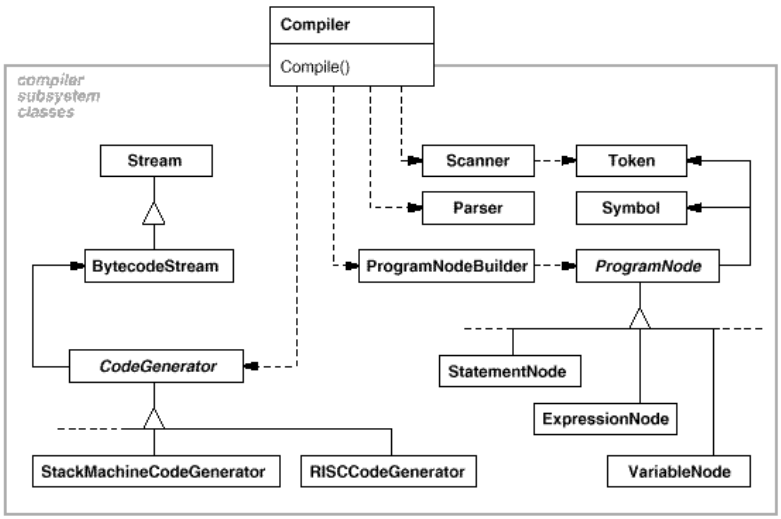
\includegraphics[scale=0.4]{5_padroes-contexto-funcional/5.2_estruturais/5.2.5_facade/facade_exemplo.png}
	\end{center}
\end{figure}


\begin{lstlisting}[caption={Façade Orientado a Objetos},label=oofacade]

class Scanner(val input : Stream){
	def Scan() : Token{
		// Retorna o token
	}
}

class Parser(){
	def Parse(scanner : Scanner, 
		builder : ProgramNodeBuilder) : Tree[ProgramNode] {
		// Retorna a árvore de análise
	}
}

class ProgramNodeBuilder() {
	var rootNode : ProgramNode;

	// Possui os métodos para criação dos do programa

	def getRootNode() : ProgramNode{
		return rootNode;
	}
}

class CodeGenerator(var output : BytecodeStream){
	// Possui os métodos para gerar o código de máquina do programa
}

class Compiler() {
	def Compile(input : Stream) : BytecodeStream{
		val scanner = new Scanner(input);
		val programNodeBuilder = new ProgramNodeBuilder();
		val parser = new Parser();

		parser.Parse(input, programNodeBuilder);

		var output : BytecodeStream;

		val codeGenerator = new CodeGenerator(output);
		val parseTree = programNodeBuilder.getRootNode();
		parseTree.Traverse(codeGenerator);

		return output;
	}
}



\end{lstlisting}

\subsection*{Contexto Funcional}


\begin{lstlisting}[caption={Façade Funcional},label=fpfacade]
    

    
\end{lstlisting}